\chapter{HomeDS - Server}
\section{Einleitung}\label{sec:einleitung}
Im Rahmen der Diplomarbeit muss neben dem XIBO-Server ein weiterer Server eingesetzt werden. Es handelt sich um einen Java Enterprise Edition Server. Aufgrund der hohen Komplexität des Signage-Servers aber dünn dokumentierten API-Schnittstellen und begrenzten technischen Möglichkeiten, muss ein weiterer Server eingesetzt werden. Dieser wird für die Kommunikation zwischen Signage Server und Applikation-Client erleichtern. Der JavaEE Server verwendet die Funktionen des Signage Servers und baut diese meist aus, sodass neue Funktionen entstehen können.

\begin{figure}[H]
\centering
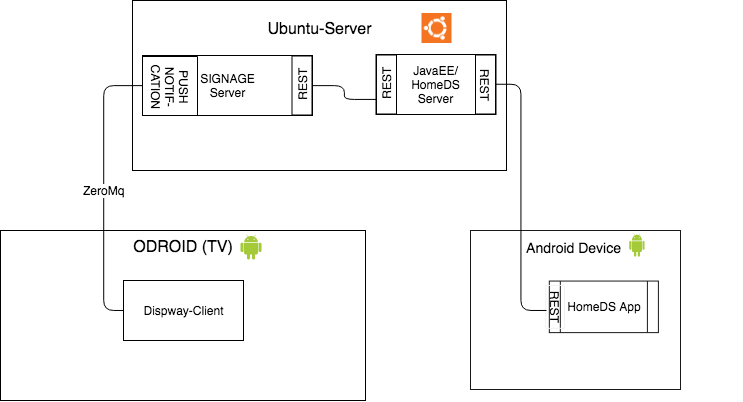
\includegraphics[width=1\textwidth]{images/08_HomeDsWeb/SystemArch.png}
\caption{Systemarchitektur - HomeDS}
\label{img:systemarchitektur}
\end{figure}
 
\section{Anforderungen an den HomeDS Server}\label{sec:homeds}
Der JavaEE Server soll die verschiedenen komplizierten Abläufe des XIBO-Servers vereinfachen. Die Zugriffe mittels REST die eigentlich direkt auf den XIBO laufen sollen, werden über den JavaEE Server verwaltet. Siehe Abblidung \ref{img:systemarchitektur}. Das heißt, der Java Enterprise Server empfängt REST Zugriffe, verarbeitet diese entsprechend und tätigt dann REST Abfragen auf den XIBO Server dieser benachrichtigt dann mittels PUSH Notifications über ZeroMQ die Display Clients. Das Einsetzten eines weiteren JavaEE Server hat insofern einen großen Vorteil, da die komplizierte Authentifizierungen wegfällt. Des Weiteren können ohne Probleme neue Funktionen hinzugefügt und neue Anforderungen flexibel erfüllt werden. Aufgrund dieser Vorgehensweise müssen Grundfunktionen des Signage Servers nicht erneut programmiert werden. Es werden lediglich über die möglichen API-Schnittstellen neue Funktionen und Erweiterungen speziell für die benötigten Anwendungsfälle erstellt. Siehe Abbildung \ref{img:xiboengine}

\begin{figure}[H]
\centering
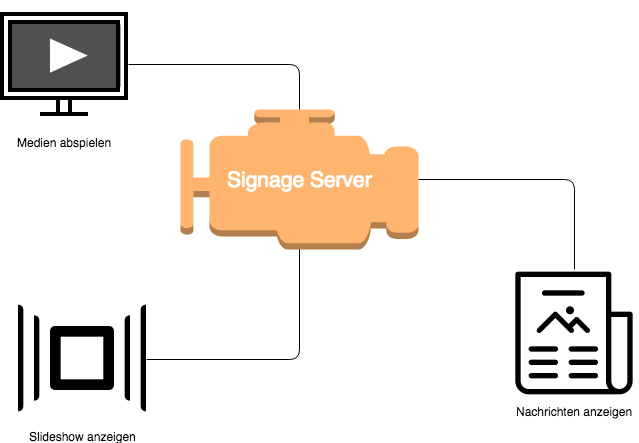
\includegraphics[width=1\textwidth]{images/08_HomeDsWeb/SignageEngine.png}
\caption{Signage Server unsere Enginge - HomeDS}
\label{img:xiboengine}
\end{figure}
 
\section{Komponenten des HomeDS Server}\label{sec:homedscomponents}
Der Server ist in Java programmiert und verfügt über eine eigene MySQL Datenbank. Über REST Schnittstellen sind die Funktionen des Servers verfügbar. Des Weiteren befindet sich auf dem Server auch eine JSF Weboberfläche also Java Server Faces Komponente. Der ganze Server wird auf einem Wildfy Application Server mittels Continous Integration deployed. 
 
\section{Funktionen des JavaEE}
\subsection{Weboberfläche des JavaEE}\label{sec:javaeejsfweb}
Die HTL Leonding kann mithilfe von einem Signage Server und der HomeDS Webapplikation Projektvideos der Schüler auf einen gewünschten Bildschirm anzeigen.  Zum Beispiel kann das Sekretariat der HTL Leonding neuste Nachrichten oder Informationen in kürzester Zeit in der ganzen Schule auf allen Bildschirmen im System anzeigen lassen.

\begin{figure}[H]
\centering
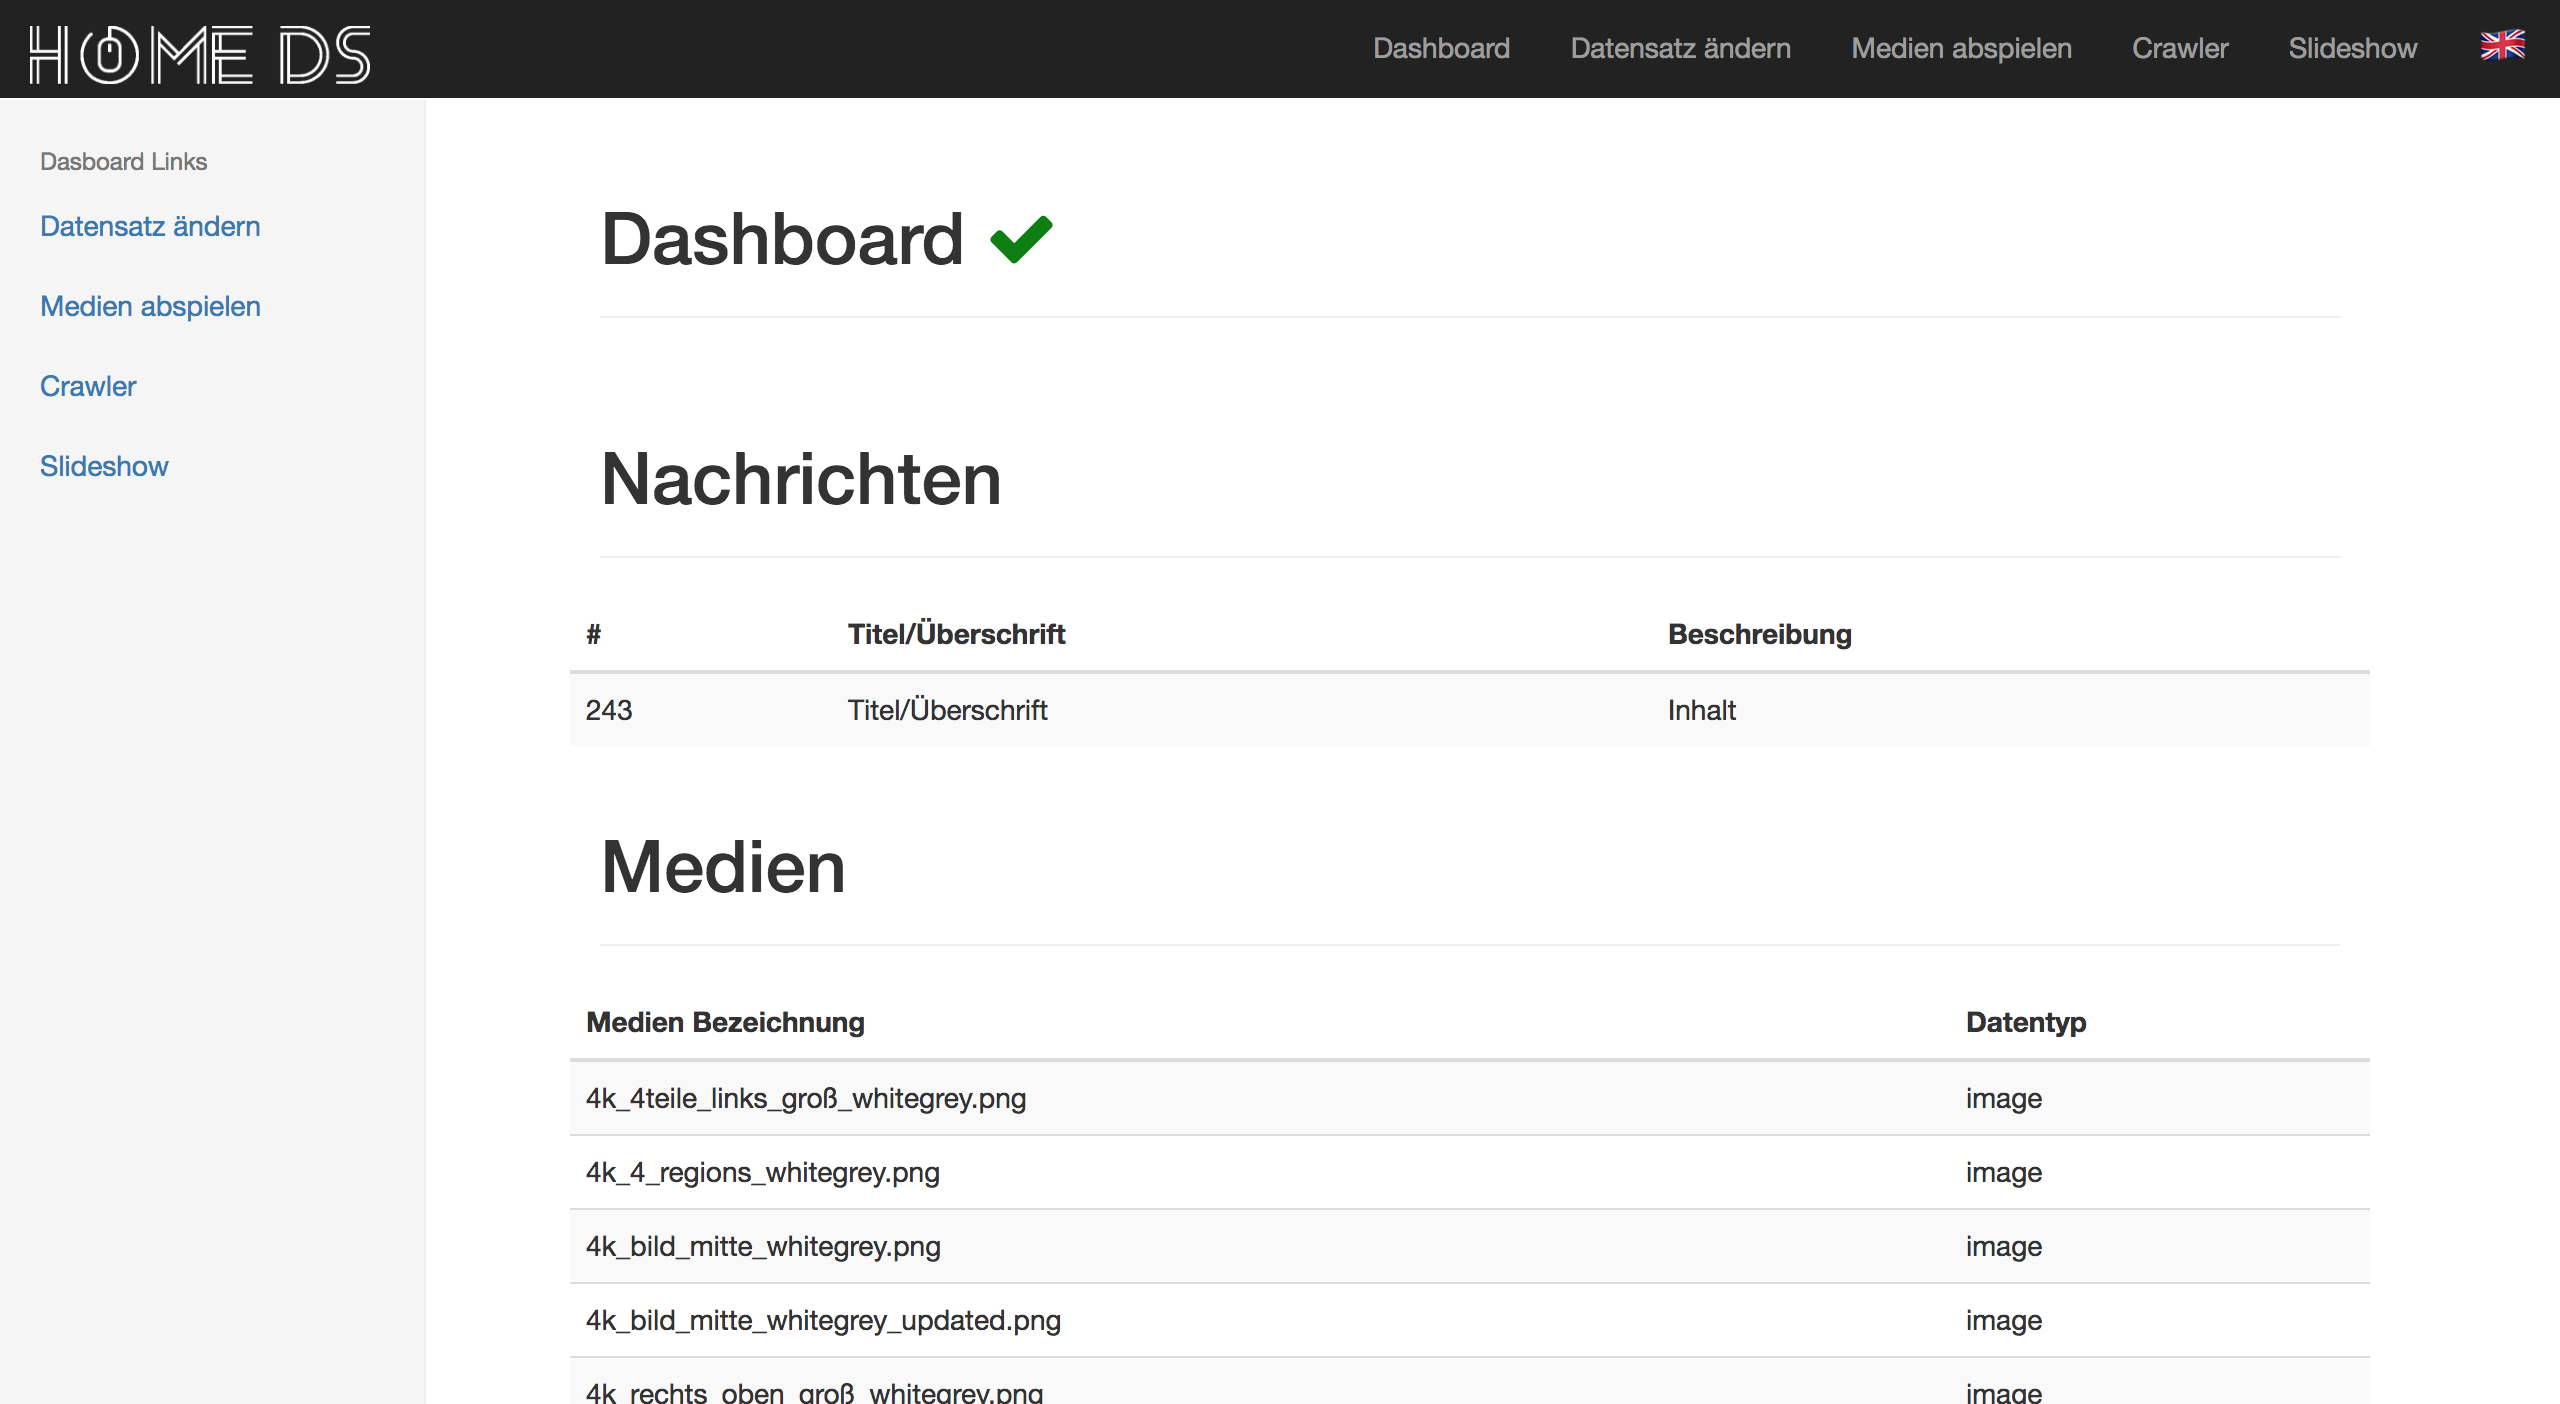
\includegraphics[width=1\textwidth]{images/08_HomeDsWeb/DashboardHomeDsWeb.png}
\caption{Startseite - HomeDsWeb}
\label{img:Startseite}
\end{figure}

Unsere Weboberfläche ist Responsive gestaltet und mithilfe von Java Server Faces mit BootsFaces realisiert worden. Das Bootsfaces Framework stellt fertige Komponenten zur Verfügung wie Buttons, Listen, Forms etc. Dabei wurde Bootstrap als Vorbild hergenommen.

Es war wichtig die Oberfläche so zu gestalten, dass diese übersichtlich und leicht zu bedienen ist. Das Designen wurde in enger Zusammenarbeit mit dem zukünftigen Benutzern der Software ausgearbeitet. Als Vorbild fungierte das Designe eines Cockpit in einem Flugzeug wo vielen Funktionen direkt bei der Hand liegen müssen und trotzdem alles übersichtlich gestaltet ist. In der Abbildung \ref{img:Startseite} ist das Dashboard abgebildet. 
Hier erkennt man nun, dass es sich um die Kommandozentrale der Applikation handelt, von dieser Seite aus kann man über eine Top-Navigationsleiste oder eine Left Sidebar Navigation zu allen Funktionen der Website gelangen. 

Um den Nutzer immer ein Feedback über den aktuellen Status der Verbindung vom XIBO zu JavaEE Server zu geben, wird bei Erfolgreicher Verbindung ein grünes Häkchen visualisiert, versehen mit eine Tooltip. Oder bei keiner Verbindung zum Server ein rotes ''X'' dargestellt wie in der Abbildung  \ref{img:NoConnection}.

\begin{figure}[H]
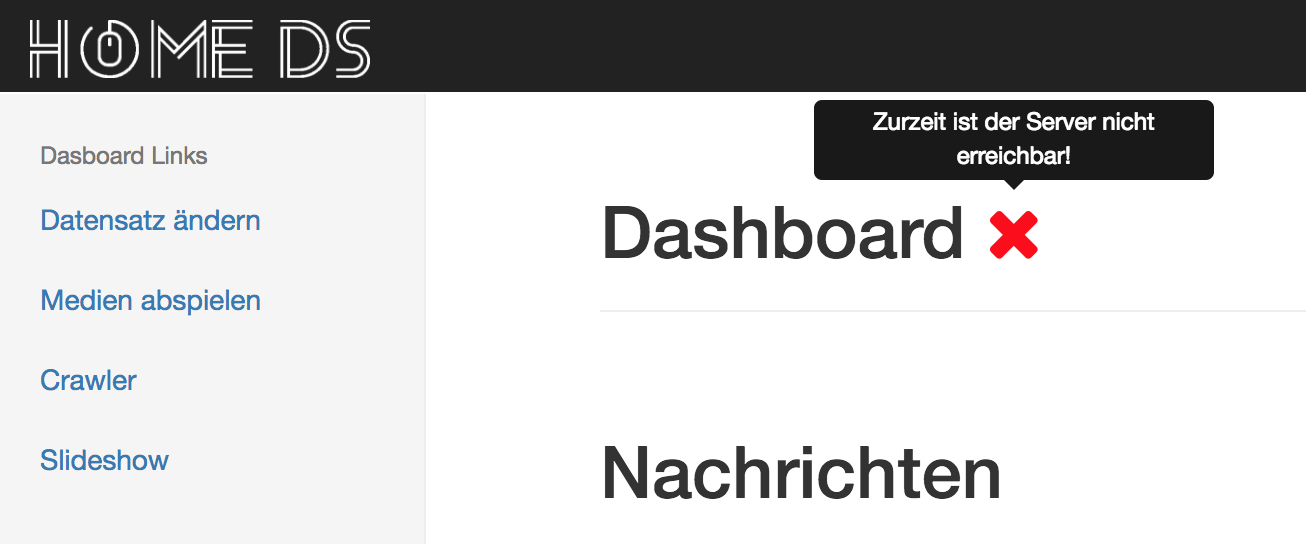
\includegraphics[width=1\textwidth]{images/08_HomeDsWeb/DashboardNoConnection.png}
\caption{Keine Verbindung zum XIBO - HomeDsWeb}
\label{img:NoConnection}
\end{figure}

\subsection{Nachrichten Pakete ändern - HomeDS Web}\label{sec:homedswebdataset}
Die ''Datensatz ändern'' Funktion auch genannt Nachrichten Pakete ändern, DataSet bearbeiten oder Nachrichten Pakete bearbeiten kann über das Dashboard erreicht werden.
Die Aufgabe der ''Nachrichten Paket ändern'' Funktion ist es ein DataSet zu ändern, hinzufügen oder zu löschen. Diese Seite besteht grob gesagt aus 2 Teilen. Diese 2 Teile können bei Bedarf auf- und zugeklappt werden.

Teil 1 kümmert sich um das Anzeigen aller DataSets in einer Responisve Komponente die ''DataTable'' genannt wird in der Bibliothek vom Bootsfaces Framework. Im DataTable ist es möglich die Anzahl der angezeigten Elemente pro Seite zu begrenzen oder erweitern,  die einzelnen Spalten sortieren dabei kann man zwischen ab- oder aufsteigend wählen und durch die verschiedenen Spalten einer Zeile eine Suche durch zu führen. 


\begin{figure}[H]
\centering
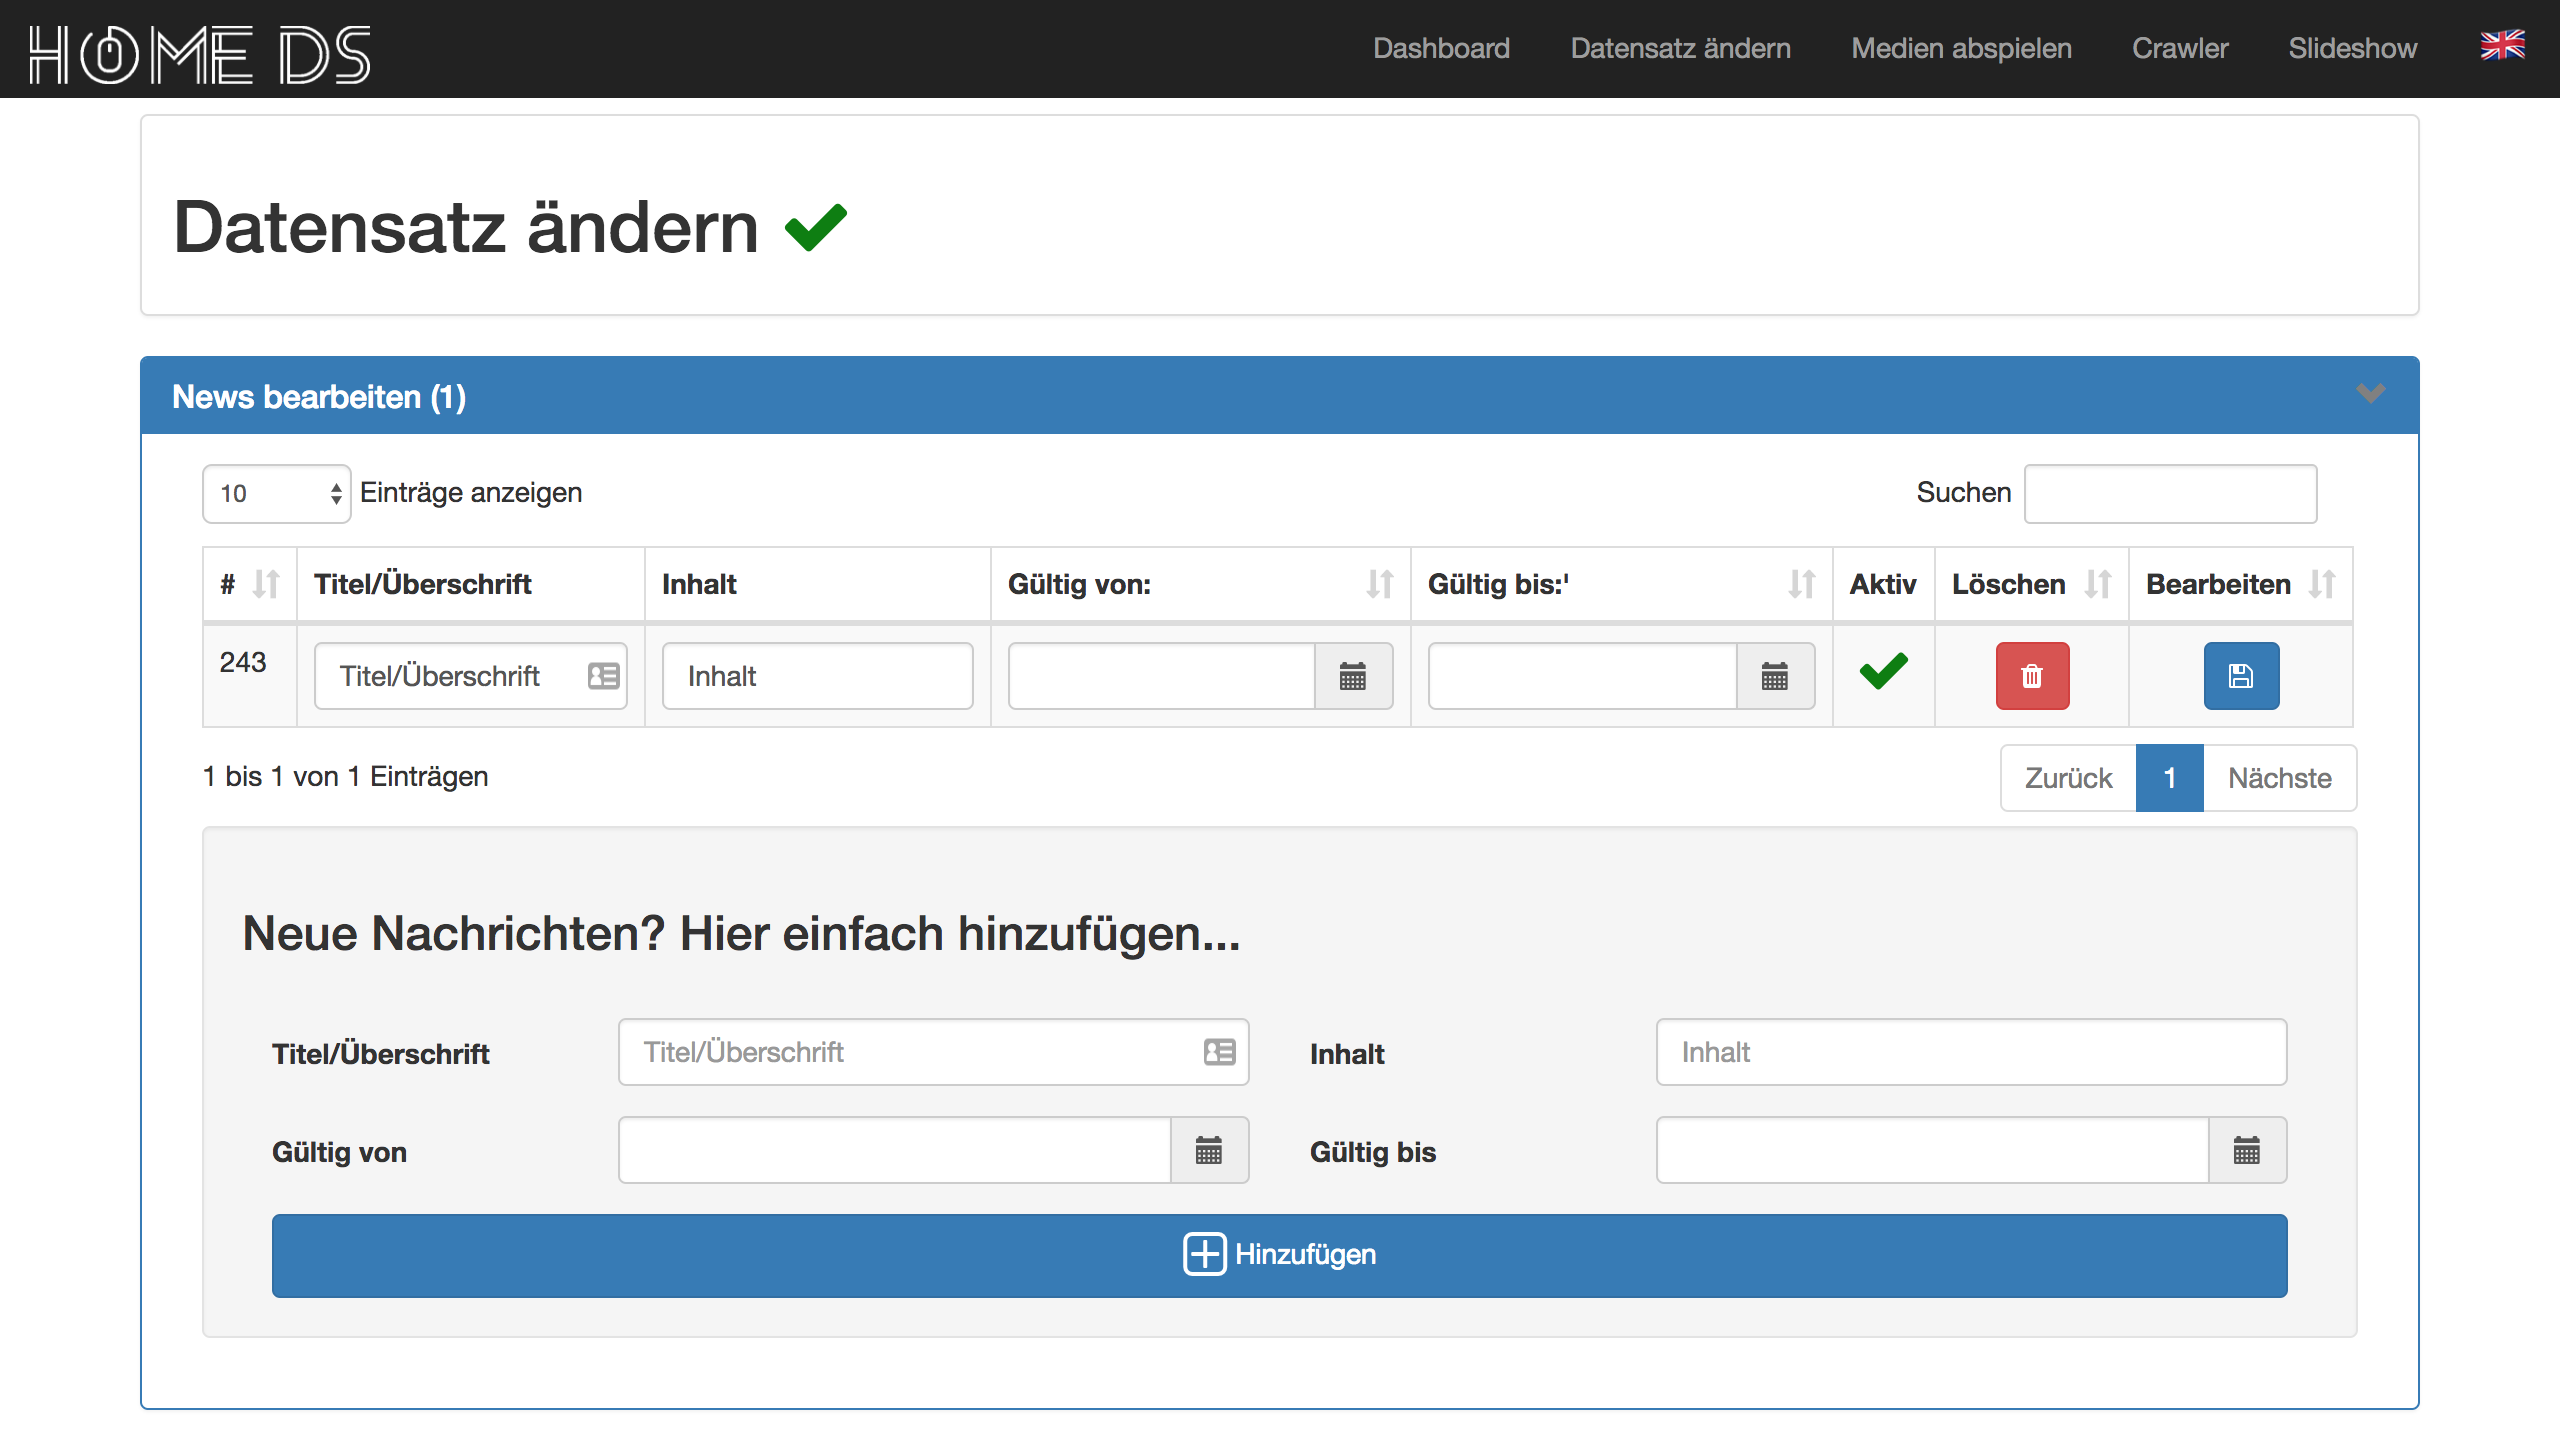
\includegraphics[width=1\textwidth]{images/08_HomeDsWeb/NachrichtenPaket.png}
\caption{Nachrichten ändern - HomeDsWeb}
\label{img:changenews}
\end{figure}


Es ist auch durch die editierbaren Textfelder und DatePicker möglich die DataSets zu ändern. Durch klicken auf den Speichern Button wird die Änderung des einzelnen DataSets bestätigt. Durch klicken auf den roten Löschen Button wird das Nachrichtenpaket gelöscht falls es aktiv war wird es auch aus dem XIBO System entfernt. Die Logik ist im \pageref{sec:datasetexpiredate} nochmals genauer erklärt. 

Der zweite Teil der ''Datensatz ändern'' Seite ist das Hinzufügen von Nachrichtenpaketen, dabei ist der Titel und der Inhalt der Nachricht natürlich erforderlich. Bei nicht eingeben von Start Datum des Nachrichtenpakets wird davon ausgegangen das es sofort in den XIBO gespeichert werden soll und somit auf aktiv gesetzt wird. Andersrum wenn kein Ablaufdatum eingegeben wird, wird das DataSet solange angezeigt bis entweder ein Ablaufdatum im Nachhinein hinzugefügt wird oder es manuell einfach wieder gelöscht wird.

Nach jeder Aktion wird die Webseite mit einer Loading Animation versehen und der Nutzer bekommt dann ein Feedback ob die jeweilige Operation erfolgreich oder fehlgeschlagen ist. Siehe Abbildung \ref{img:feedback}

\begin{figure}[H]
\centering
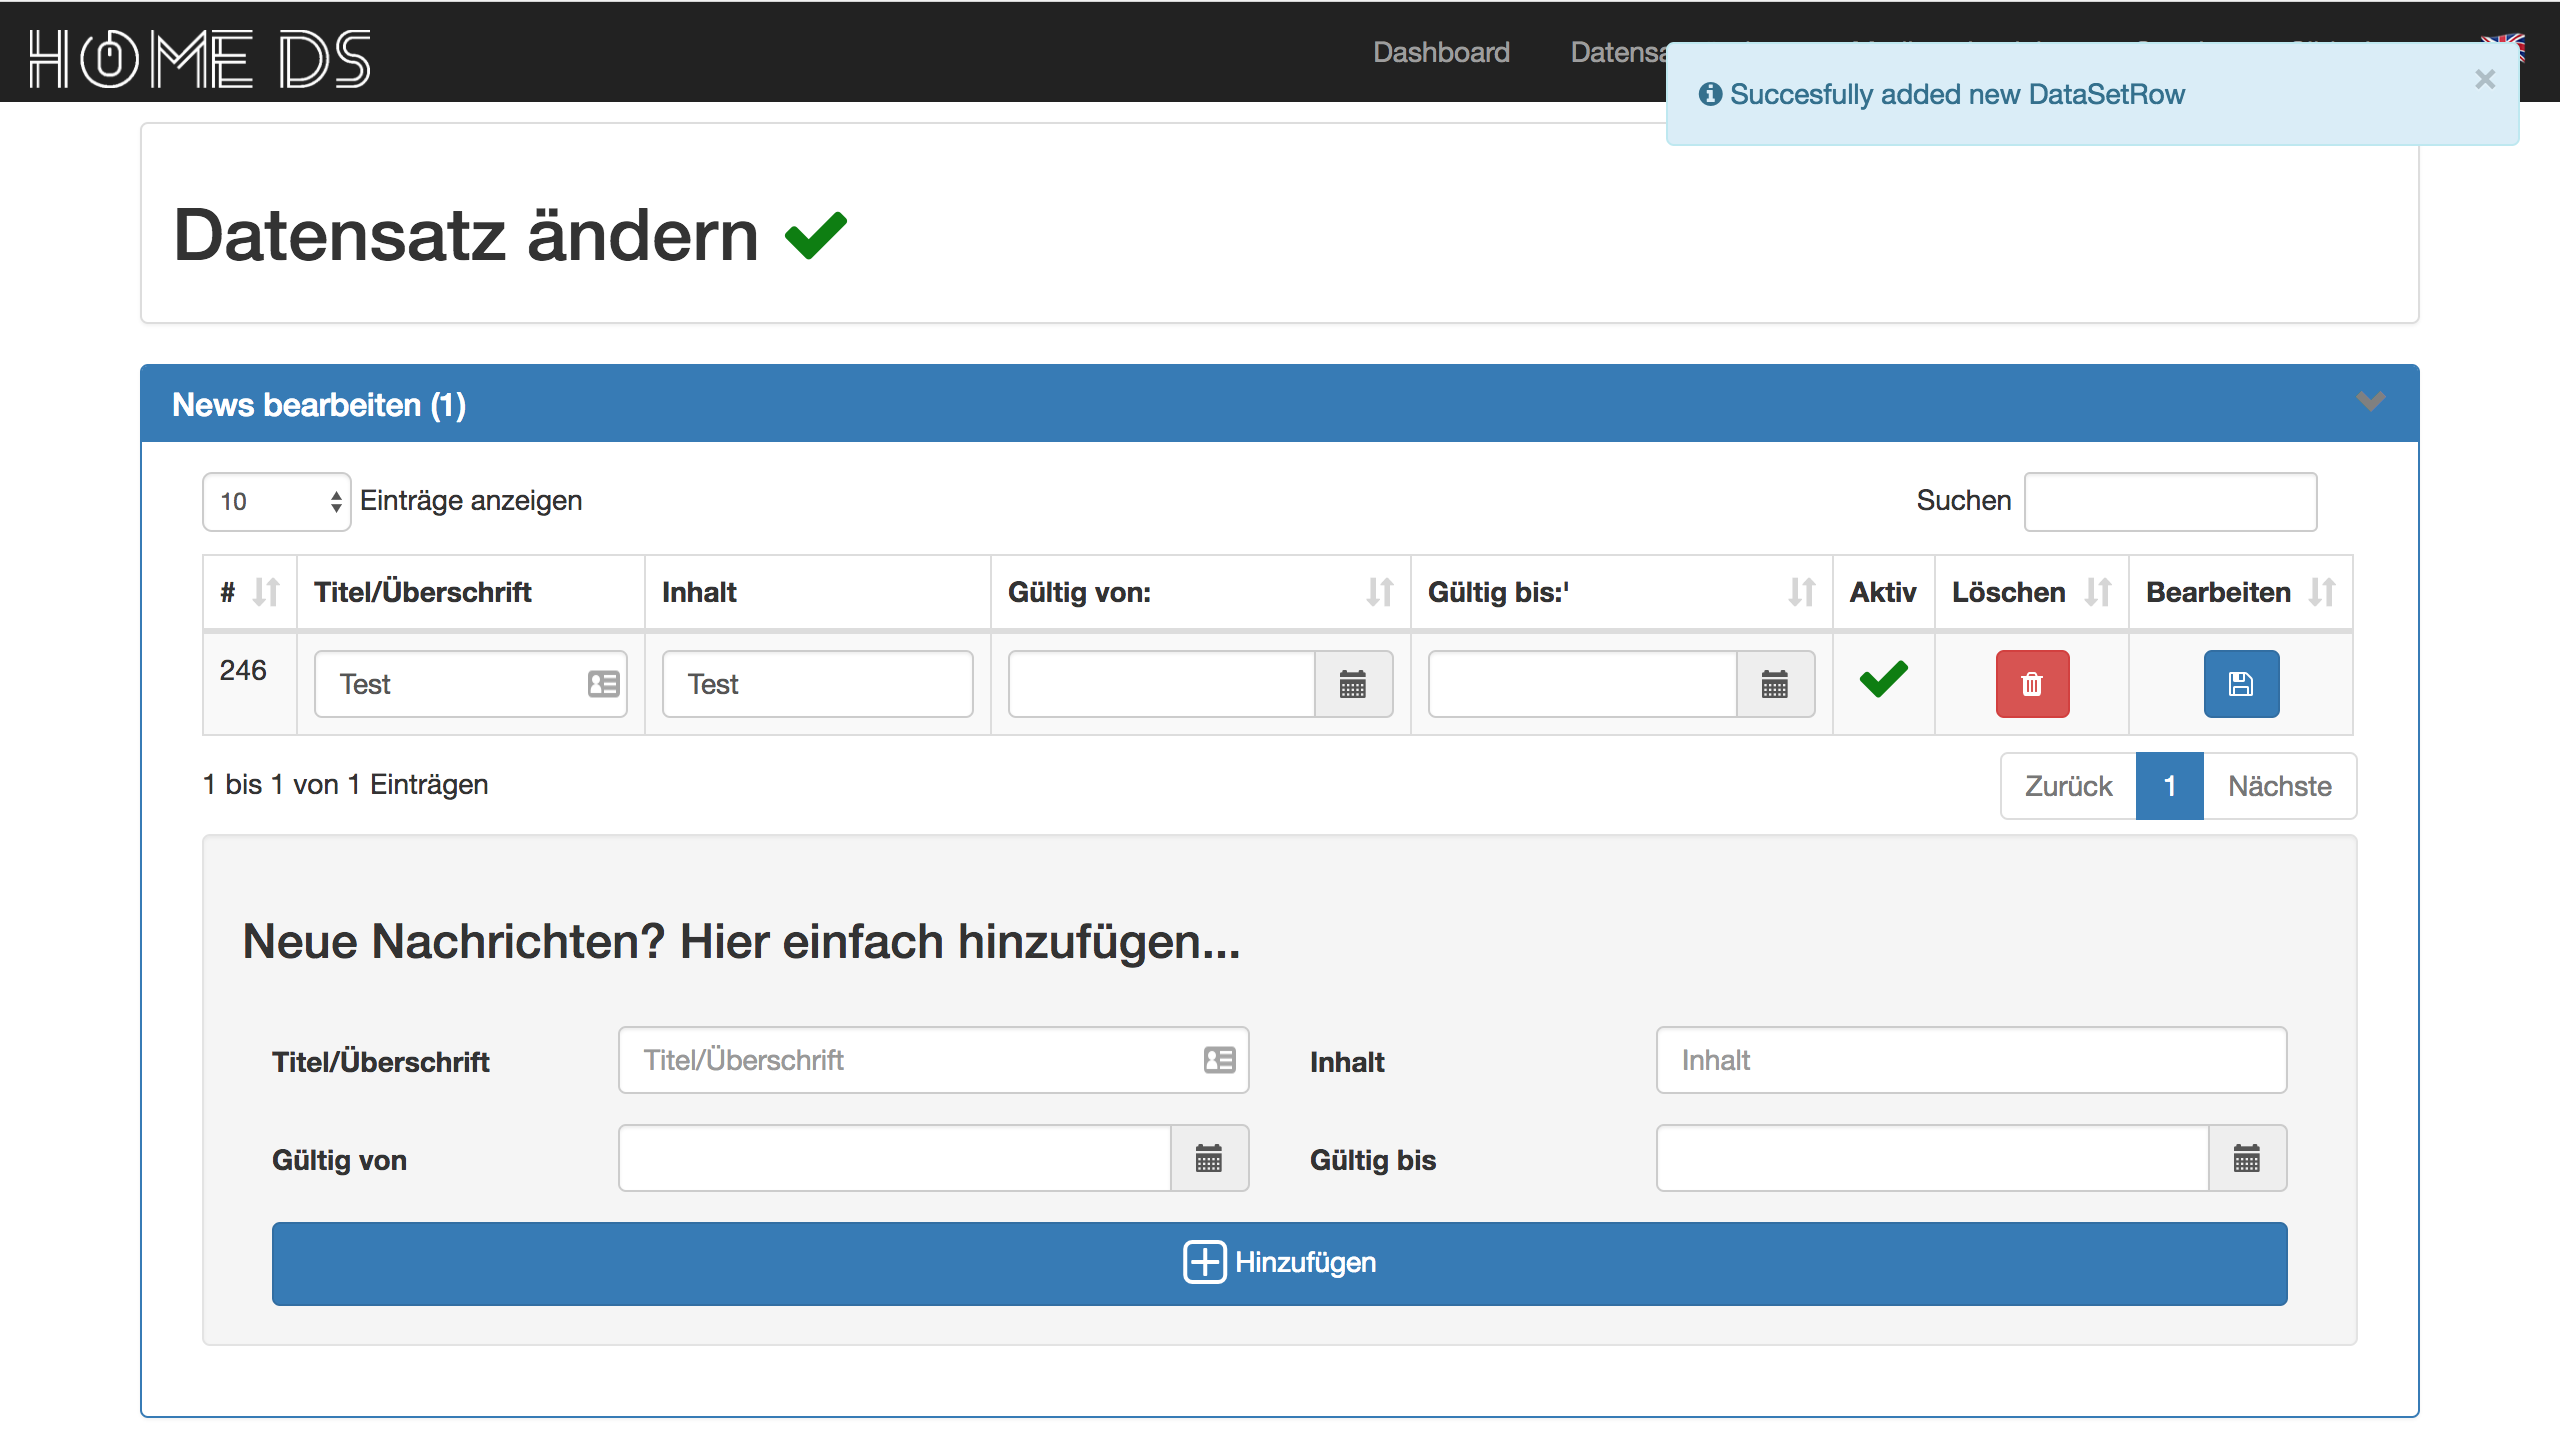
\includegraphics[width=1\textwidth]{images/08_HomeDsWeb/Message.png}
\caption{Feedback - HomeDsWeb}
\label{img:feedback}
\end{figure}

\subsection{Medien abspielen - HomeDS Web}\label{sec:playmedia}
Eine weitere Funktion ist das Abspielen von Medien die im XIBO hinterlegt sind. Es soll dem Nutzer eine einfache und übersichtliche Oberfläche zur Verfügung gestellt werden die Medien abspielt. Der Nutzer kann auf dieser Seite dann den Bildschirm auswählen auf den das gewünschte Video abgespielt werden sollen. Des Weiteren soll verhindert werden das der Nutzer stundenlang sein gewolltes Video aus der XIBO Bibliothek heraussuchen muss. Diese Herausforderung wurde mithilfe von Schlagworten und einer Schlagwort-Wolke gelöst. Auch werden nur Medien Formate wie Foto und Video aus der XIBO Bibliothek geladen.

\begin{figure}[H]
\centering
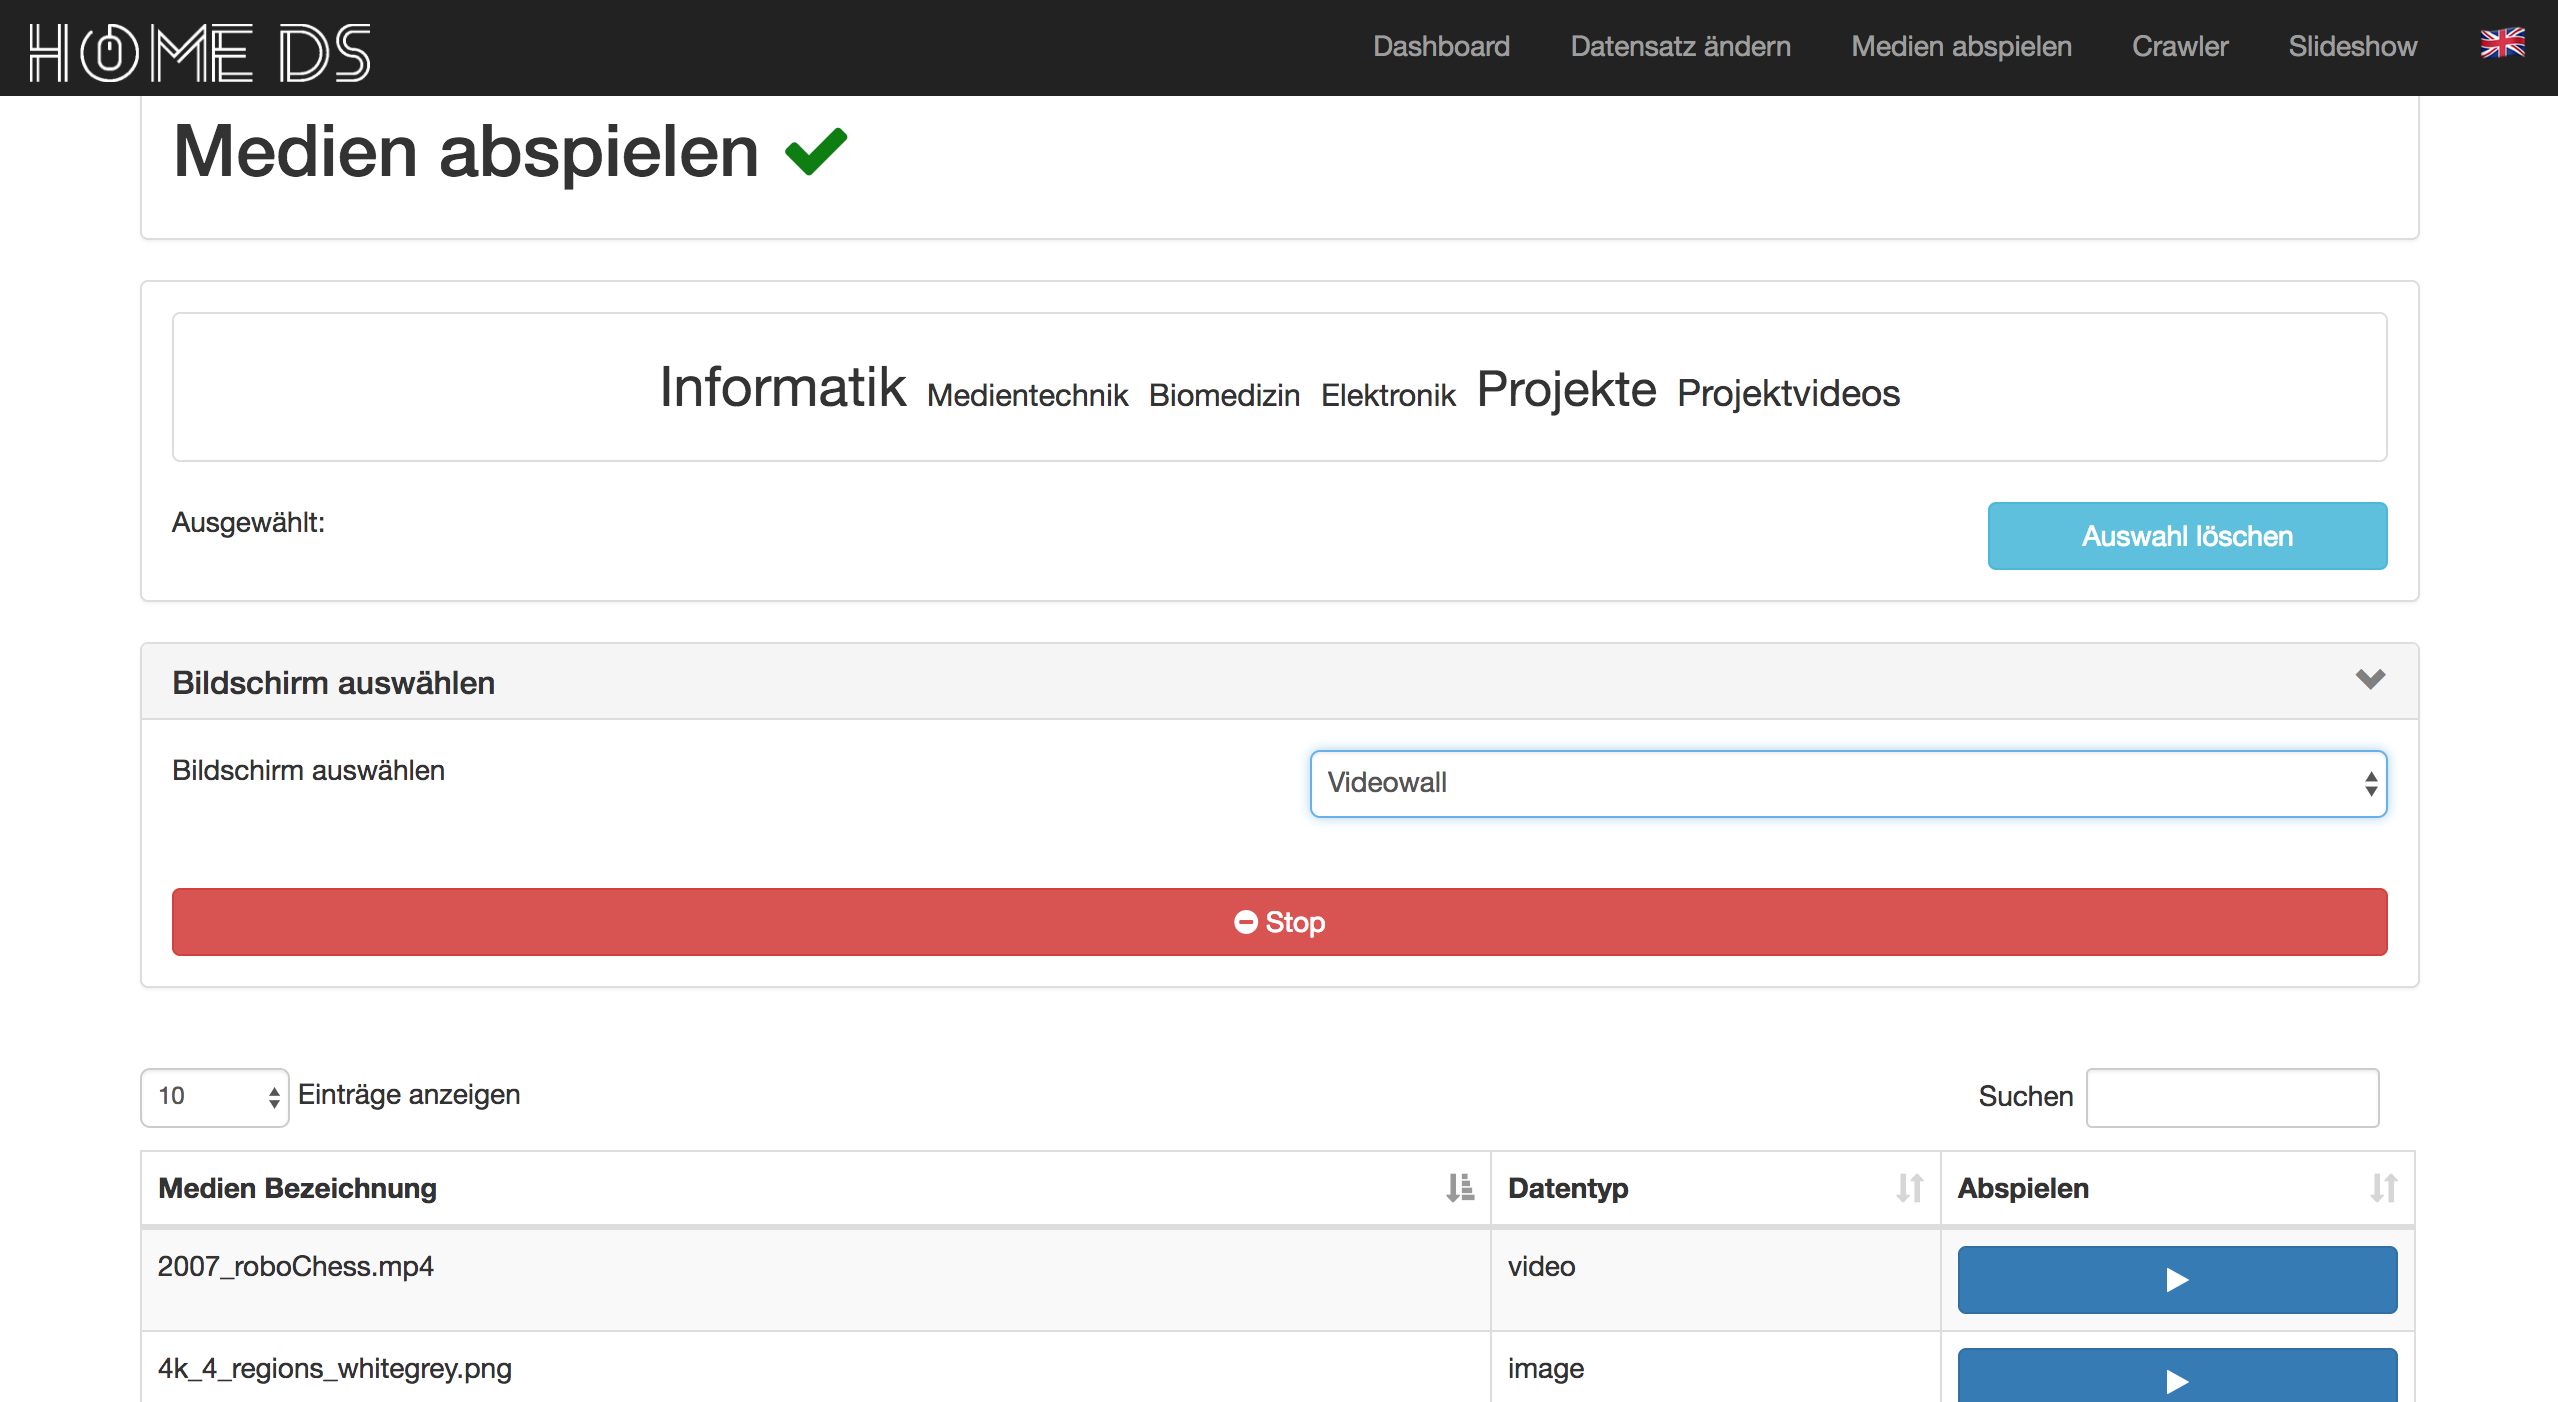
\includegraphics[width=1\textwidth]{images/08_HomeDsWeb/PlayMediaOverview.png}
\caption{Medien abspielen - HomeDsWeb}
\label{img:playmedia}
\end{figure}

Die Medien im XIBO müssen mit einem Schlagwort versehen werden. Diese Schlagwörter können sein, die jeweilige Abteilung also Informatik, Medientechnik oder Elektronik. Es kann sich aber auch um ein Projekt oder sonstiges handeln. Die Wahl der Schlagworte bleibt dem Nutzer überlassen.  Siehe Abbildung \ref{img:playmedia}

Mithilfe dieser Tags wollen wir dem Nutzer die Suche nach dem richtigen Video erleichtern. Der Nutzer bekommt die Möglichkeit einer dieser Tags auf der HomeDs Weboberfläche auszuwählen, daraufhin werden nur die Videos mit dem entsprechendem Tag angezeigt.

Nachdem der Nutzer sein Schlagwort und den gewünschten Bildschirm ausgewählt und auch schon das Video oder Foto gefunden hat, welches er anzeigen möchte muss er nur den Play-Button drücken. Nach der Meldung das dieses Element erfolgreich abgespielt wurde erscheint es innerhalb weniger Sekunden auf dem gewünschten Bildschirm. Das Video wird bis zum Ende abgespielt und danach wieder das vorige Layout hergestellt. Wenn ein weiteres Element abgespielt wird während dem Element 1 wird das Video 1 abgebrochen und das Element 2 wird abgespielt.

Neben dem Abspielen gibt es auch die Stop Funktion, diese soll sofort wieder das Layout ,welches vor dem Abspielen des Videos angezeigt wurde, wiederherstellen.


\subsection{Structure Crawler - HomeDS Web}\label{sec:javaeestructurecrawler}
Für das Verstehen des Aufbaus eines Layouts war es die Aufgabe einen sogenannten StructureCrawler zu erstellen. Dieser soll den JSON Aufbau eines Layouts ausgeben. Durch diese Funktion ist es für uns möglich gewesen das ganze Signage System zu verstehen und zu verwenden. Dabei kann die ID eines Layouts oder der Name eingegeben werden und der Crawler liefert dann alle enthaltenen Entitäten des jeweiligen Layouts im JSON Format. Dieser JSON kann mithilfe der ''Copy to Clipboard'' Funktion in die Zwischenablage kopiert werden.

Der Crawler ist eigentlich nur ein REST-Zugriff der sich alle Layouts vom XIBO Server holt und dabei alle anderen Child-Elemente des Layouts mitschickt. Dies ist praktisch, denn es unterstützt bei dem Arbeiten mit vielen verschiedenen Elementen, die alle eindeutige Schlüssel besitzen.

\begin{figure}[H]
\centering
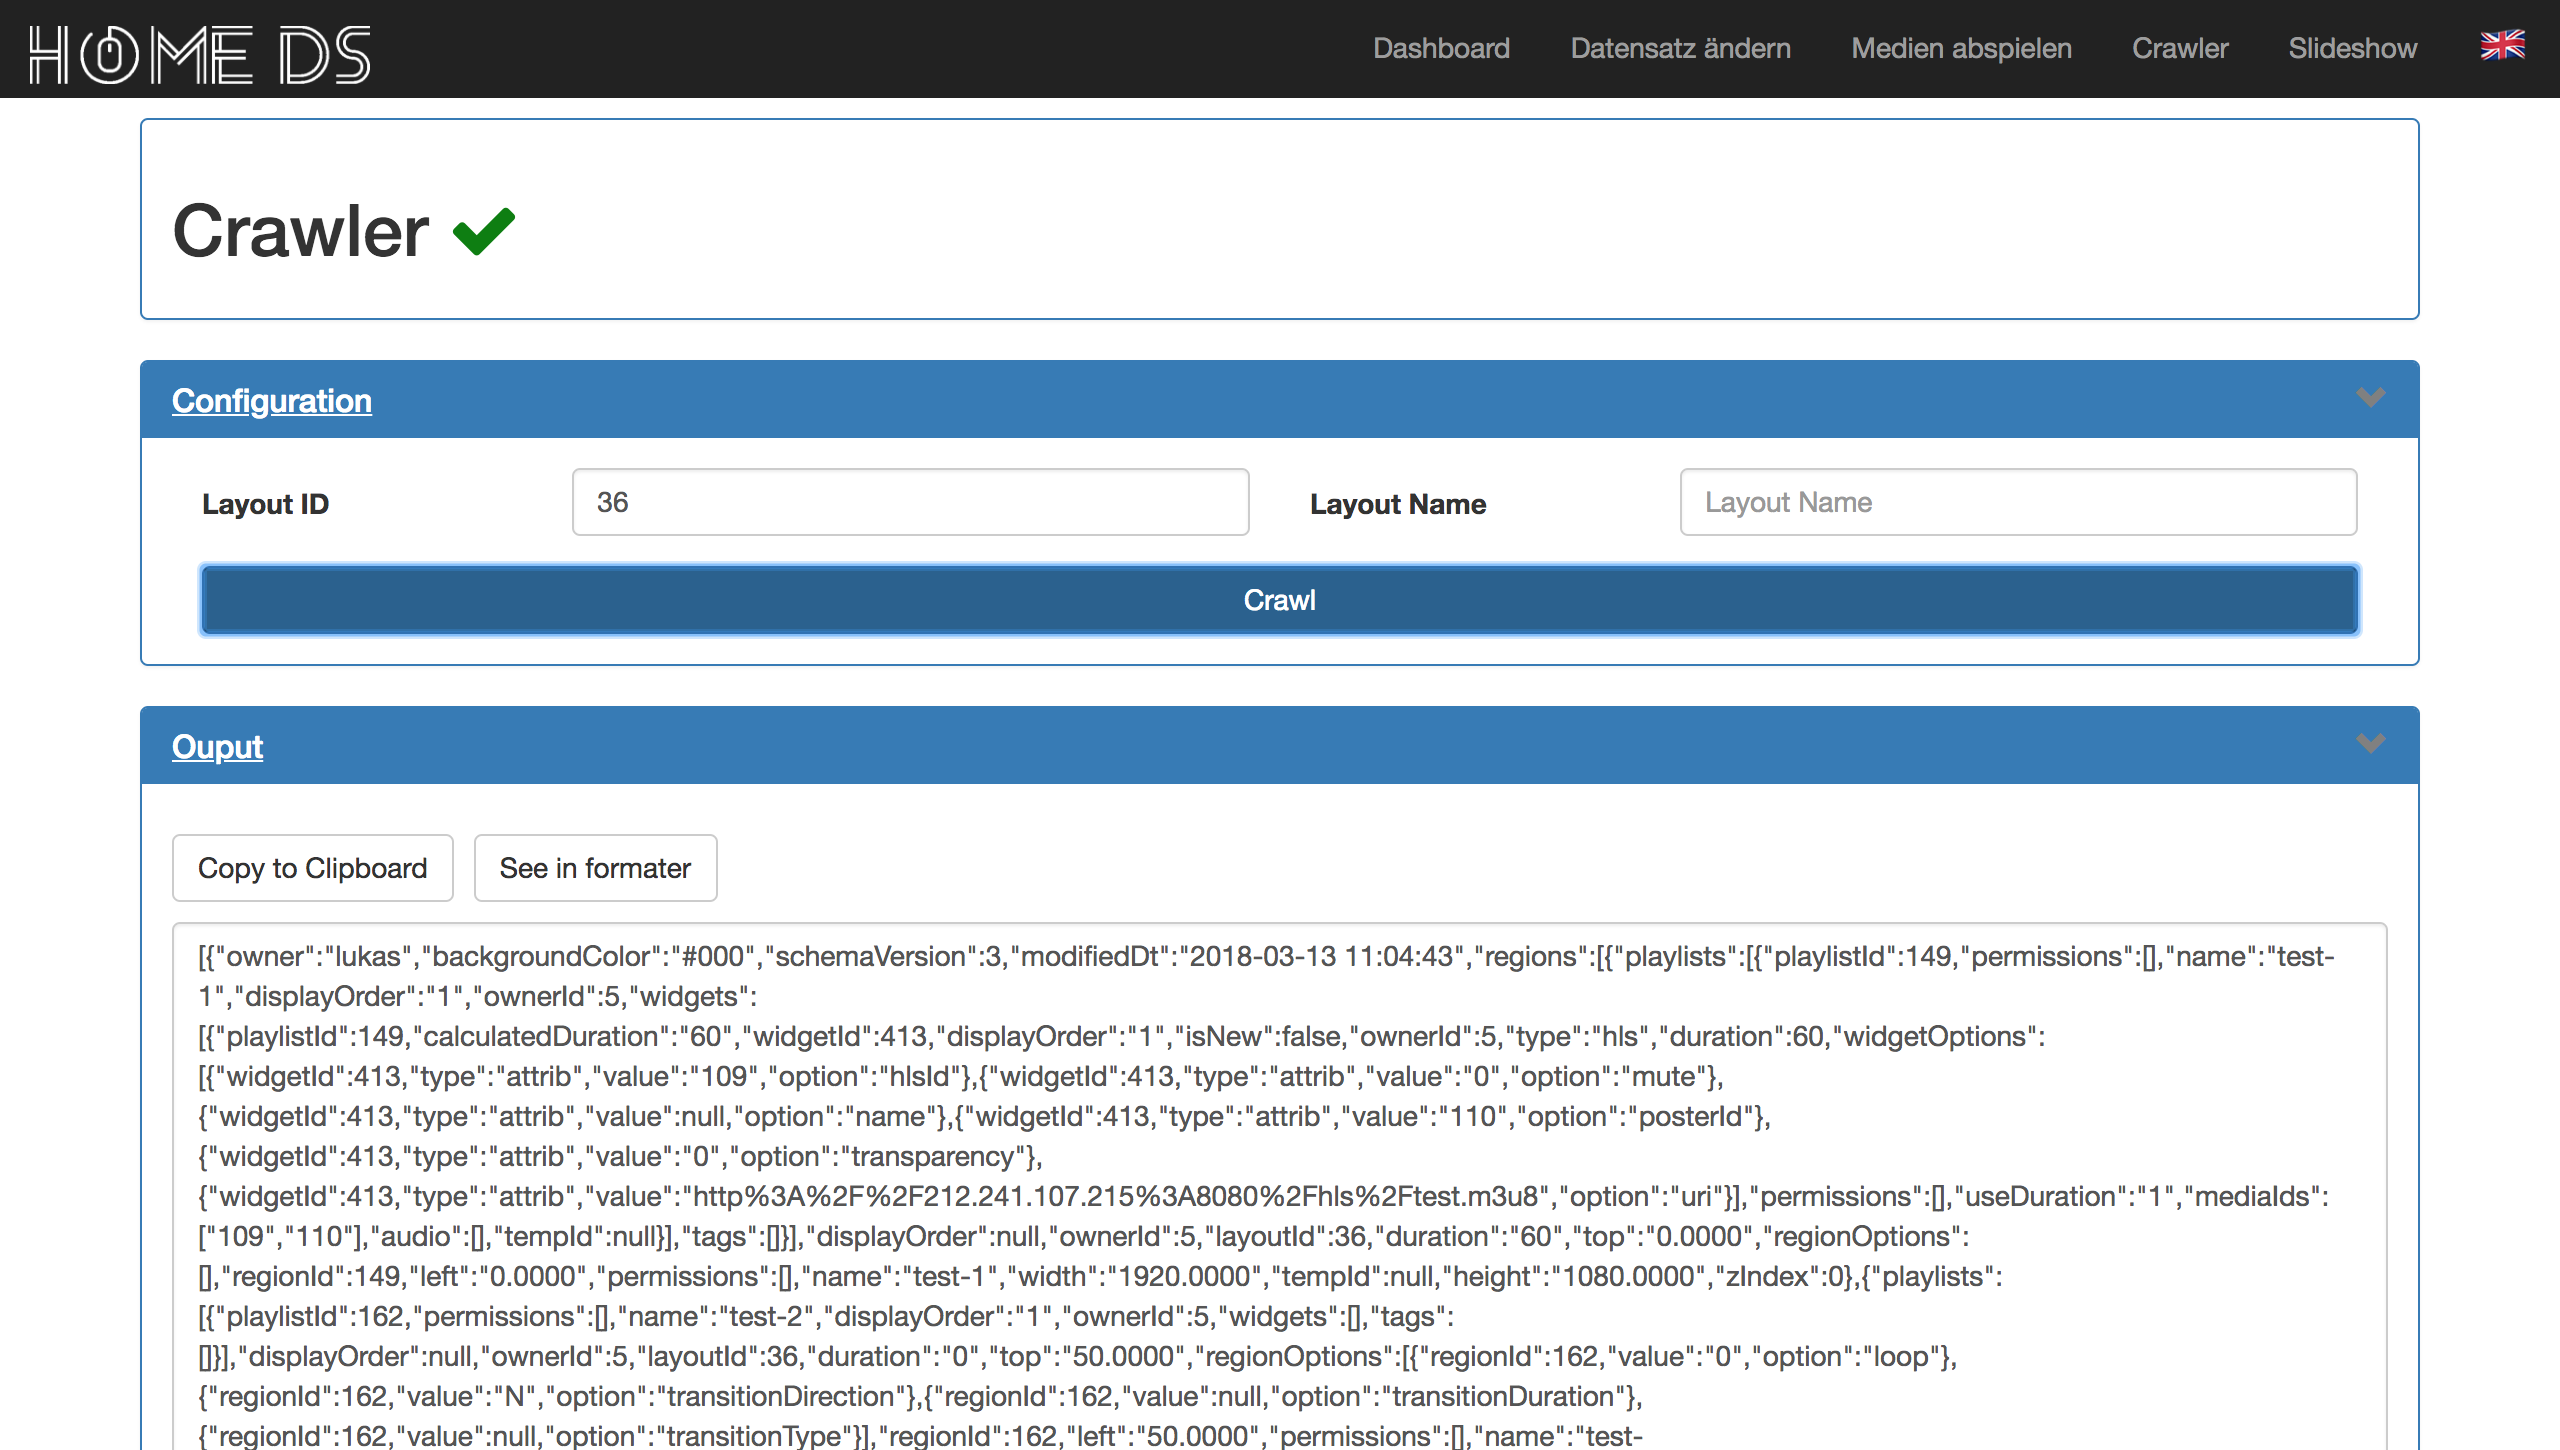
\includegraphics[width=1\textwidth]{images/08_HomeDsWeb/Crawler.png}
\caption{Crawler - HomeDsWeb}
\label{img:crawler}
\end{figure}

\subsection{HomeDS Server Slideshow - HomeDS Web}\label{sec:homedsslideshow}
Eine weitere Funktion des HomeDs Servers ist das Abspielen von Medien ohne diese in den XIBO hochladen zu müssen. Dabei handelt es sich um eine Website die Bilder aus dem lokalen Server Ordner mit einem Wechselintervall von 3 Sekunden anzeigt. 

\subsection{Internationalisierung - HomeDS Web}\label{sec:i18n}
Die Weboberfläche der HomeDS Anwendung ist vollständig übersetzt in Englisch und Deutsch. Die Sprache kann ganz leicht mit einem Klick entweder auf die Englische oder Österreichische Flagge dementsprechend geändert werden.

\begin{figure}[H]
    \centering
    \subfloat{{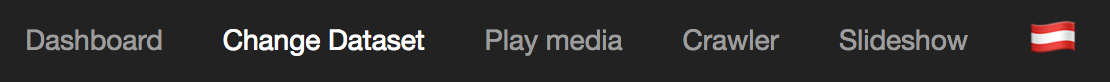
\includegraphics[width=6cm]{images/08_HomeDsWeb/austrianflag.png}}}%
    \qquad
    \subfloat{{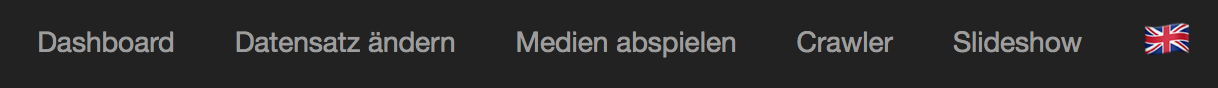
\includegraphics[width=6cm]{images/08_HomeDsWeb/britishflag.png}}}%
    \caption{Internationalisierung}
    \label{img:flags}
\end{figure}

\section{Funktionen des JavaEE - Technischer Hintergrund}
\label{sec:javaeetechnicalbackground}
Um den Benutzern die Möglichkeit zu geben die Funktionen des Servers zu nutzen wurde auch eine Webapplikation erstellt. Die Entscheidung mit welcher Technologie die Weboberfläche programmiert werden soll ist schnell auf JSF gefallen. Diese hat nämlich viele Vorteile wie zum Beispiel die Platzformunabhängigkeit und auch schnelle Entwicklung im Vergleich zu anderen Clients. Mit JSF wird nämlich über eine Managed Bean direkt im XHTML auf die Funktionen des Servers zugegriffen somit sind keine REST Zugriffe nötig.

\subsection{Nachrichten-Pakete ändern - Technisch}\label{sec:datasetexpiredatetechnical}
Der Benutzer kann Start- und Enddatum für jeden einzelnen DataSet eingeben. Erst wenn das Datum genau in diesem Zeitintervall inklusive den Grenzen liegt, wird das DataSet an den Xibo mittels API-Schnittstelle weitergegeben. Es wurde auch so programmiert, dass bei keinem Startdatum das Nachrichten Paket sofort angezeigt wird oder wenn kein Enddatum festgelegt wird, dass es bis zum Manuellen deaktivieren angezeigt wird.

\begin{lstlisting}[language=Java, caption={public void doCheckEvery24Hours()}]
if (dataset.isActive() == false && (dataset.getFromDate().minusDays(1)
        .isBefore(LocalDate.now()))) {
    try {
        //if succesfull added then set active true and add id
        if ((id=dataSetApi.addDataSetField(dataset)) > 0) {
            dataset.setDataRowId(id);
            dataset.setActive(true);
            dataSetFieldFacade.save(dataset);
        }
    } catch (NoConnectionException e) {
        // Catch Exception
    }
}
\end{lstlisting}

Die Überprüfung ob die DataSets aus der Server-Datenbank im Zeitintervall liegen, wird mithilfe der Java Annotation @Schedule jeden Tag um 01:00 Uhr durchgeführt. Falls dieses DataSet im Intervall liegt, wird dieses an den XIBO Signage Server gesendet. Diese Überprüfung beinhaltet auch das FromDate. Dies löscht bei überschreiten des Bis-Datums das DataSet aus dem Digital Signage heraus. Solange das DataSet sich im XIBO befindet wird es angezeigt nach dem entfernen aus dem XIBO wird es dann auch nicht mehr angezeigt.

Falls keine Nachrichten Pakete aktiv oder im System sind werden aus dem RSS-Feed der HTL Leonding die Neuigkeiten anstatt der Nachrichten Pakete angezeigt.

\subsection{Medien abspielen - Technisch}\label{sec:playmediatechnical}
Die Medien werden per REST aus dem XIBO abgefragt dabei wird schon der Datentyp und das Schlagwort gefiltert. Es werden auch die Bildschirme die im XIBO angemeldet sind abgefragt. Wenn der Nutzer den Bildschirm ausgewählt hat und bei einem der Medien auf den ''Play Button'' gedrückt hat. Wird per REST im XIBO in einem Layout ein Widget vom Typ Bibliothek das Medium zugewiesen. Falls dies Erfolgreich verlaufen ist wird daraufhin dieses Layout wieder mittels REST in den Kalender vom ausgewähltem Bildschirm eingeplant mit einer Priorität von 20. Prioritäten sind dazu da um bei mehreren Events diese überschreiben zu können zum Beispiel wenn 2 Events gleichzeitig eingeplant sind dann wird das Event, dass eine höheren Priorität besitzt angezeigt.

Das heißt, wenn gerade Nachrichten vom Sekretariat auf einem Bildschirm angezeigt werden und auf diesem Bildschirm dann Medien abgespielt werden. Hat das ''Medien abspielen'' (Priorität 20) gegenüber dem ''Nachrichten anzeigen'' (Priorität 10) Vorrang und wird abgespielt Beim Ende oder Beenden des ''Medien abspielen'' werden dann wieder die Nachrichten angezeigt.

\subsection{JavaEE mit REST}\label{sec:javaeeresttechnical}
Der Server stellt Funktionen wie Medien abspielen, Nachrichten Paket ändern, löschen, hinzufügen oder abfragen, Status abfragen und den Crawler per REST zur Verfügung.

Die REST Schnittstellen sind mithilfe von Swagger dokumentiert. \pageref{sec:javaeeandroidrestswagger}

\subsection{Swagger}\label{sec:javaeeandroidrestswagger}
Swagger wird verwendet um Funktionalität und Möglichkeit einer API übersichtlich zu gestalten. Swagger dokumentiert welche Response Code's man erwarten kann, wie bei einem POST oder PUT der Body aussehen muss oder welche Pathparams mitgegeben werden müssen oder welche nur optional sind. Dabei gibt es zwei verschiedene Arten eine REST-Dokumentation zu erstellen.

Die erste Möglichkeit wäre, mit dem Swagger Editor die Dokumentation in der JSON-Ausdruckssprache mit der Hand zu schreiben und immer wieder zu aktualisieren. Natürlich ist dies bei vielen verschiedenen GETs, POSTs, PUTs und DELETEs sehr aufwendig und mühsam.

Bei der zweiten Methode, die auch bei der Diplomarbeit zum Einsatz kommt, werden die API's automatisch von der im Projekt eingebundenen Swagger Engine erkannt. Daraus wird dann auch wieder eine JSON-File generiert, die dann mithilfe von Swagger-UI gut im Browser über eine Webseiten URL erreichbar ist.

Unsere Swagger-Dokumentation ist unter ''http://vm59.htl-leonding.ac.at:8080/homeds/swagger/swagger.html'' oder ''BASE_URL:PORT/homeds/swagger/swagger.html'' zu finden


Verweis: https://swagger.io/

\subsection{Structure Crawler - Technisch}\label{sec:structurecrawlertechnical}
Der Crawler holt sich per REST vom XIBO ein Layout mit allen Sub-Entitäten. Ohne parameter gibt XIBO aber nur das Model von Layout im JSON zurück um aber auch weitere Enitäten mit zu laden musste mit dem Querparam  ''embed='' der REST Zugriff modifiziert werden. Dabei müssen mit einem Komma getrennt, die weiteren Entitäten angegeben werden, die mit geladen werden sollen.

\begin{lstlisting}[language=Java, caption={Crawler GET Request}]
HttpURLConnection con = new RequestHelper()
                    .executeRequest(RequestTypeEnum.GET, null,
                            new RequestHelper().BASE_URL + "api/layout?" + "embed=regions,playlists,widgets,widgetOptions" + query,
                            AuthentificationHandler.getTOKEN());
\end{lstlisting}

\subsection{HomeDS Server Slideshow - Technisch}\label{sec:slideshowtechnical}
Bei der Slideshow Funktion müssen mittels einem FTP-Client die Bilder auf den vm59.htl-leonding.ac.at Server in den Ordner ''/home/vwall/images/'' hochgeladen werden. Danach werden die Medien aus dem Ordner gelesen und in einem Intervall von 3 Sekunden nach der Reihe auf einer Website abgespielt. Bei dieser Funktion wurde plain JavaScript, HTML und CSS verwendet.

\begin{lstlisting}[caption={Carousel JavaScript}]
function carousel() {
    var x = document.getElementsByClassName("mySlides");
    for (i = 0; i &lt; x.length; i++) {
    		 x[i].style.display = "none";
  	 }
     myIndex++;
   	if (myIndex > x.length) {
   		myIndex = 1
    	 }
      x[myIndex - 1].style.display = "block";
      setTimeout(carousel, 3000); //Change image every 3 seconds
}
\end{lstlisting}
